\documentclass[a4paper,12pt,titlepage]{article}
\usepackage[utf8]{inputenc}
\usepackage{graphicx} % Required for inserting images
\usepackage[spanish,es-tabla]{babel}
\usepackage[none]{hyphenat}
\usepackage[justification=centering]{caption}
\usepackage{subcaption}
\usepackage{amssymb, amsmath}
\usepackage{gensymb}
\usepackage{fancyhdr}
\usepackage{wrapfig}


\title{Modos normales}
\author{Gonzalo Bastos González}

\usepackage[a4paper]{geometry}
\geometry{top=2cm, bottom=2.0cm,left=2cm, right=2cm}

\begin{document}

\begin{center}
    \textbf{\Large Modos normales en medios continuos}
\end{center}

\begin{center}
    \textbf{Gonzalo Bastos González}
\end{center}

\section{Modos normales en una cuerda vibrante}

En primer lugar vamos a estudiar los modos normales en una cuerda vibrante de longitud $L=167,5\pm0,5\; cm$. Colgaremos varias masas $m_i$ de la cuerda que ejercerán una tensión constante y aplicaremos sobre la cuerda una fuerza vertical oscilante de frecuencia $\nu$ con $s(\nu)=0,1\;Hz$. Aumentaremos la frecuencia hasta encontrar los modos normales en los que se produce resonancia. Para las 6 primeras frecuencias de resonancia, que obedecen la expresión $\nu_n=n\nu_1$ con $n\in \mathbb{N}$, anotaremos las distancias entre nodos $d$ con $s(d)=0,5\;cm$, que nos servirán para calcular la longitud de onda $\lambda$:

\begin{equation}
    \lambda_n = 2d_n \Rightarrow s(\lambda_n) =2s(d_n)
\end{equation}

Para el valor de $d_n$ de cada modo normal tomaremos el valor medio de las distancias entre nodos medidas en el laboratorio. Calcularemos también el período ($T$) de la cuerda para cada frecuencia de resonancia:

\begin{equation}
    T = \frac{1}{\nu_n} \Rightarrow s(T) = \frac{s(\nu_n)}{\nu_n^2}
\end{equation}

Estos datos nos van a servir para determinar la velocidad de propagación de la onda para cada $m_i$, que verifica la relación:

\begin{equation}
    \lambda_n=c_iT_N
    \label{v propagación}
\end{equation}

Realizaremos un ajuste para las 5 masas con las que trabajamos que nos permitirá obtener su velocidad de propagación $c_i$. Obtendremos valores diferentes en función de la masa que cuelgue de la cuerda, por lo que podemos ver la influencia de la tensión de la cuerda ($\tau$) en la velocidad de propagación de las ondas. La relación a la que obedecen estas magnitudes es:

\begin{equation}
    c_i^2 = \rho_l^{-1}\tau_i \quad (\tau=m_ig;\,s(\tau)=gs(m_i))
    \label{dens lineal}
\end{equation}

Siendo $\rho_l$ la densidad lineal de la cuerda, que obtendremos a partir de un ajuste y compararemos con el valor real. A continuación expondremos los datos obtenidos experimentalmente con los que realizaremos los ajustes:

\begin{table}[h!]
    \centering
    \begin{tabular}{|c|c|c|c|c|c|c|}
    \hline
    $n$ & $\nu_n(Hz)$ & $d(m)$& $\lambda(m)$ & $s(\lambda)(m)$ &$T(s)$ & $s(T)(s)$ \\ \hline
    1  & 14,2 & 1,675 & 3,350 & 0,01 & 0,07042  & 0,00050  \\ \hline
    2  & 28,5 & 0,838 & 1,675 & 0,01 & 0,03509  & 0,00012  \\ \hline
    3  & 43,5 & 0,558 & 1,117 & 0,01 & 0,022989 & 0,000053 \\ \hline
    4  & 57,5 & 0,419 & 0,838 & 0,01 & 0,017391 & 0,000030 \\ \hline
    5  & 71,4 & 0,335 & 0,670 & 0,01 & 0,014006 & 0,000020 \\ \hline
    6  & 83,6 & 0,279 & 0,558 & 0,01 & 0,011962 & 0,000014 \\ \hline
    \end{tabular}
    \caption{Datos para $m_1=100\;g$}
    \label{masa1}
    \end{table}

\begin{table}[h!]
    \centering
    \begin{tabular}{|c|c|c|c|c|c|c|}
        \hline
        $n$ & $\nu_n(Hz)$ & $d(m)$& $\lambda(m)$ & $s(\lambda)(m)$ &$T(s)$ & $s(T)(s)$ \\ \hline
        1 & 20,1 & 1,675 & 3,350 & 0,01 & 0,04975   & 0,00025   \\ \hline
        2 & 40,2 & 0,838 & 1,675 & 0,01 & 0,024876  & 0,000062  \\ \hline
        3 & 60,3 & 0,558 & 1,117 & 0,01 & 0,016584  & 0,000028  \\ \hline
        4 & 80,2 & 0,419 & 0,838 & 0,01 & 0,012469  & 0,000016  \\ \hline
        5 & 100,0  & 0,335 & 0,670 & 0,01 & 0,010000  & 0,000010  \\ \hline
        6 & 120,0  & 0,279 & 0,558 & 0,01 & 0,0083333 & 0,0000069 \\ \hline
        \end{tabular}
        \caption{Datos para $m_2=198\;g$}
        \label{masa2}
        \end{table}

\begin{table}[h!]
    \centering
        \begin{tabular}{|c|c|c|c|c|c|c|}
            \hline
            $n$ & $\nu_n(Hz)$ & $d(m)$& $\lambda(m)$ & $s(\lambda)(m)$ &$T(s)$ & $s(T)(s)$ \\ \hline
            1 & 31,7  & 1,675 & 3,350 & 0,01 & 0,031546  & 0,000099  \\ \hline
            2 & 63,6  & 0,838 & 1,675 & 0,01 & 0,015723  & 0,000025  \\ \hline
            3 & 95,0    & 0,558 & 1,117 & 0,01 & 0,010526  & 0,000011  \\ \hline
            4 & 126,7 & 0,419 & 0,838 & 0,01 & 0,0078927 & 0,0000062 \\ \hline
            5 & 158,9 & 0,335 & 0,670 & 0,01 & 0,0062933 & 0,0000040 \\ \hline
            6 & 190,7 & 0,279 & 0,558 & 0,01 & 0,0052438 & 0,0000027 \\ \hline
        \end{tabular}
    \caption{Datos para $m_3=504\;g$}
    \label{masa3}
\end{table}

\begin{table}[h!]
    \centering
        \begin{tabular}{|c|c|c|c|c|c|c|}
            \hline
            $n$ & $\nu_n(Hz)$ & $d(m)$& $\lambda(m)$ & $s(\lambda)(m)$ &$T(s)$ & $s(T)(s)$ \\ \hline
                1 & 37,4  & 1,675 & 3,350 & 0,01 & 0,026738  & 0,000072  \\ \hline
                2 & 74,7  & 0,838 & 1,675 & 0,01 & 0,013387  & 0,000018  \\ \hline
                3 & 112,0   & 0,558 & 1,117 & 0,01 & 0,0089286 & 0,0000080 \\ \hline
                4 & 149,4 & 0,419 & 0,838 & 0,01 & 0,0066934 & 0,0000045 \\ \hline
                5 & 187,3 & 0,335 & 0,670 & 0,01 & 0,0053390 & 0,0000029 \\ \hline
                6 & 224,2 & 0,279 & 0,558 & 0,01 & 0,0044603 & 0,0000020 \\ \hline
            \end{tabular}
            \caption{Datos para $m_4=704\;g$}
            \label{masa4}
\end{table}

\begin{table}[h!]
    \centering
    \begin{tabular}{|c|c|c|c|c|c|c|}
    \hline
    $n$ & $\nu_n(Hz)$ & $d(m)$& $\lambda(m)$ & $s(\lambda)(m)$ &$T(s)$ & $s(T)(s)$ \\ \hline
    1 & 44,5  & 1,675 & 3,350 & 0,01 & 0,022472  & 0,000051  \\ \hline
    2 & 89,0    & 0,838 & 1,675 & 0,01 & 0,011236  & 0,000013  \\ \hline
    3 & 133,4 & 0,558 & 1,117 & 0,01 & 0,0074963 & 0,0000056 \\ \hline
    4 & 177,9 & 0,419 & 0,838 & 0,01 & 0,0056211 & 0,0000032 \\ \hline
    5 & 222,4 & 0,335 & 0,670 & 0,01 & 0,0044964 & 0,0000020 \\ \hline
    6 & 266,9 & 0,279 & 0,558 & 0,01 & 0,0037467 & 0,0000014 \\ \hline
    \end{tabular}
    \caption{Datos para $m_5=1002\;g$}
    \label{masa5}
    \end{table}

\newpage

A partir de estos datos podemos hacer una regresión lineal simple a la Ec.\ref{v propagación}. Los resultados obtenidos para cada masa se pueden ver en la siguiente gráfica:

\newpage

\begin{figure}[h!]
    \centering
    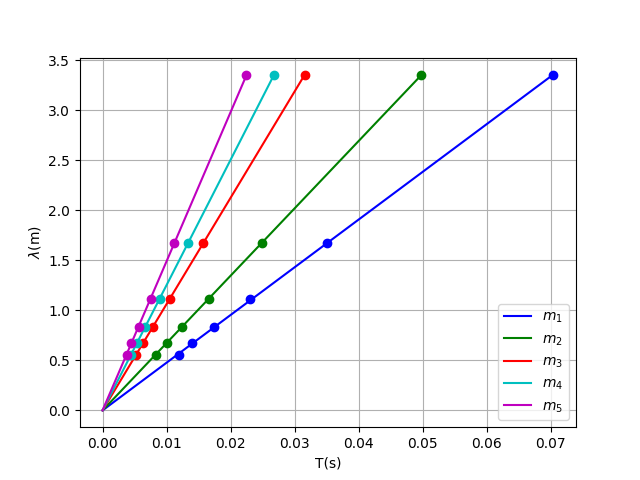
\includegraphics[width=0.75\linewidth]{Images/landa_T.png}
    \caption{Regresiones lineales $\lambda-T$ ($\lambda_n=c_iT_n$)}
\end{figure}

La pendiente de nuestras rectas de regresión $y=bx$ coincide con la velocidad de la propagación de la onda $c_i$ para cada masa $m_i$, por tanto los valores obtenidos para las velocidades de propagación son:

\begin{table}[h!]
    \centering
    \begin{tabular}{|c|c|c|c|c|c|}
        \hline
        $m(g)$ & $m_1=100$ & $m_2=198$ & $m_3=504$ & $m_4=0,704$ & $m_5=1002$ \\ \hline
        $c_i(m\cdot s^{-1})$ & 47,69 & 67,315 & 106,255 & 125,246 & 149,066 \\ \hline
        $s(c_i)(m\cdot s^{-1})$ & 0,14 & 0,034 & 0,061 & 0,039 & 0,012 \\ \hline
        $r$ & 0,99997 & 0.9999993 & 0.9999991 & 0.9999997 & 0.99999998 \\ \hline
    \end{tabular}
    \caption{Velocidades de propagación obtenidas a partir del ajuste por mínimos cuadrados}
\end{table}

Una vez conocidas las velocidades de propagación de las ondas podemos verificar la relación (\ref{dens lineal}) y obtener la densidad lineal de la cuerda a partir de un ajuste por mínimos cuadrados a una recta $y=bx$ donde $b$ se corresponde con $\rho_l^{-1}$. Los datos empleados para el ajuste son:

\begin{table}[h!]
    \centering
    \begin{tabular}{|c|c|c|c|c|c|}
        \hline
        $m(g)$ & $m_1=100$ & $m_2=198$ & $m_3=504$ & $m_4=0,704$ & $m_5=1002$ \\ \hline
        $c_i^2(m^2\cdot s^{-2})$ & 2273,928 & 4531,3113 & 11290,1645 & 15686,5533 & 22220,58558 \\ \hline
        $s(c_i^2)(m^2\cdot s^{-2})$ & 0,020 & 0,0012 & 0,0037 & 0,0015 & 0,00015 \\ \hline
        $\tau=mg(N)$ & 0,9800 & 1,9404 & 4,9392 & 6,8992 & 9,8196 \\ \hline
    \end{tabular}
    \caption{Velocidades de propagación obtenidas a partir del ajuste por mínimos cuadrados}
\end{table}

La incertidumbre de la tensión $\tau$ la obtenemos por propagación y es la misma para todas las masas:

\begin{equation}
    \tau = mg \Rightarrow s(\tau) = s(m)g = 0,0098\; N
\end{equation}

El ajuste realizado es una regresión lineal simple ya que consideramos la incertidumbre de $c^2$ como constante, al ser muy pequeña en comparación con los valores de $c^2$. Los resultados obtenidos fueron:

\begin{figure}[h!]
    \centering
    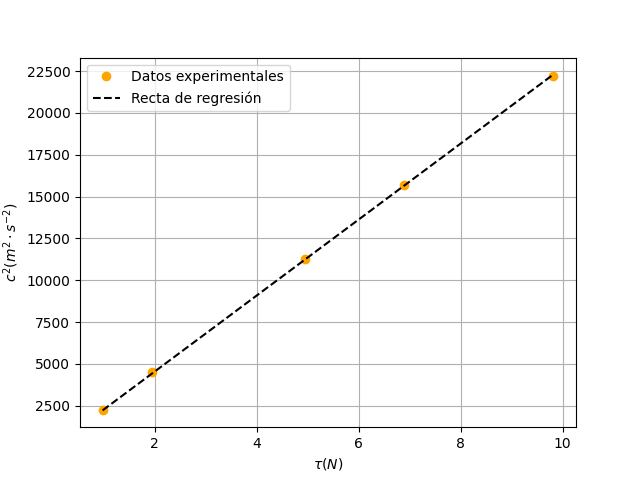
\includegraphics[width=0.75\linewidth]{Images/c_tau.png}
    \caption{Regresión lineal $c^2-\tau$ ($c^2=\rho_l^{-1}\tau$)}
\end{figure}

\begin{equation}
    \begin{gathered}
        b = 2271,0\; m\cdot kg^{-1} \Rightarrow \rho_l = \frac{1}{b} = 0,0004403 \; kg\cdot m^{-1}\\
        s(b) = 6,6\; m\cdot kg^{-1} \Rightarrow s(\rho_l) = \frac{s(b)}{b^2} = 0,0000013 \;kg\cdot m^{-1} \\
        r = 0.99998
    \end{gathered}
\end{equation}

La densidad volumétrica del cable era un dato ya conocido antes de empezar la práctica ($\rho_v = 7850 \; kg\cdot m^{-3}$) por lo que podemos obtener su diámetro y compararlo con una medición directa de este empleando las densidades que conocemos:

\begin{equation}
    \rho_l = \frac{m}{l} \quad \rho_v = \frac{m}{V} = \frac{m}{\pi r^2 l}
\end{equation}

Tomando que $d=2r$ y despejando podemos obtener la siguiente expresión para el diámetro de nuestra cuerda:

\begin{equation}
    d = 2\sqrt{\frac{\rho_l}{\pi \rho_v}} \Rightarrow s(d)=\frac{s(\rho_l)}{\pi \rho_v}\frac{1}{\sqrt{\frac{\rho_l}{\pi \rho_v}}}
\end{equation}

Tras hacer los cálculos obtenemos el siguiente valor para el diámetro:

\begin{equation}
    d = 2,6725 \pm 0,00039 \;mm
\end{equation}

Si comparamos ese valor con el real ($0,26\pm 0,01 \;mm$) podemos ver que están muy próximos y coinciden dentro de sus rangos de incertidumbre.

\newpage

\section{Estudio de la polarización}

En esta parte de la práctica realizamos un análisis cualitativo del fenómeno de la polarización. Tomamos la masa $m_2=198\;g$ sometida a una fuerza que provocaba oscilaciones en el primer modo fundamental ($n=1$). A continuación comenzamos a aumentar el voltaje, que hasta ahora se había mantenido constante y observamos su influencia en la forma en que la cuerda oscilaba. 

\par Para valores de voltaje pequeños las oscilaciones tenían lugar en el plano vertical, como observamos durante toda la práctica. A partir de valores de unos $2,5\;V$ comenzamos a observar un engrosamiento de la cuerda, comenzaba la polarización y las oscilaciones en el plano horizontal. Observamos que con esta nueva forma de oscilar al ver a trasluz podíamos diferenciar elipses cuya excentricidad decrecía a medida que aumentaba el voltaje. Por último, con voltajes de alrededor de unos $15\;V$ pudimos ver que las elipses eran ya más bien circunferencias durante algunos segundos, aunque terminaban siendo elipses otra vez. 


\section{Figuras de Chladni}

En esta última parte de la práctica estudiamos los efectos de resonancia en un medio continuo de dos dimensiones, una placa cuadrada. Para ello someteremos a nuestra placa cuadrada a una vibración de frecuencia creciente para buscar sus modos normales en los que se produce resonancia. Iremos aumentando la frecuencia $\nu$ con un voltaje inicial pequeño de unos $5\;V$ hasta que comenzamos a percibir movimiento en la arena. En este momento se empezará a producir resonancia y, para acelerar el proceso, aumentaremos el voltaje considerablemente. Las figuras observadas tras este proceso se denominan figuras de Chladni.

\par La resonancia en un medio continuo de dos dimensiones sigue un patrón ligeramente diferente a la resonancia en una dimensión observada para la cuerda continua. En un dimensión los modos normales de la cuerda seguían la siguiente relación:

\begin{equation}
    \nu_n = n\nu_1
\end{equation}

Donde $\nu_1$ es la frecuencia del primer armónico. En un medio en dos dimensiones perfectamente cuadrado la frecuencia para los modos normales obedece a la siguiente relación\footnote{French, A. P. (2012). Vibraciones y ondas. Reverte.}:

\begin{equation}
    \nu_{12} =c \sqrt{n_1^2+n_2^2} 
\end{equation}

Donde $c$ es una constante relacionada con la geometría de la placa. Si expresamos los modos normales en función del primer armónico obtenemos la siguiente expresión:

\begin{equation}
    \nu_{12} = \nu_1 \sqrt{n_1^2+n_2^2}
\end{equation}

Los enteros $n_1$ y $n_2$ son los enteros que caracterizan los modos normales, siendo para una membrana de dos dimensiones dos enteros y no uno como en la cuerda continua. Esto implica que las frecuencias modales no son múltiplos enteros de $\nu_1$, como anteriormente. Es por esto que en nuestro experimento realizamos un estudio simplemente cualitativo de los modos en la placa cuadrada, pues las relaciones anteriores aplican a medios ideales y son difíciles de verificar.

\par El primer armónico aparece para $\nu=205\pm1\;Hz$ y los nodos siguen una forma que está entre un rombo y una circunferencia, como podemos ver en la siguiente imagen:

\begin{figure}[h!]
    \centering
    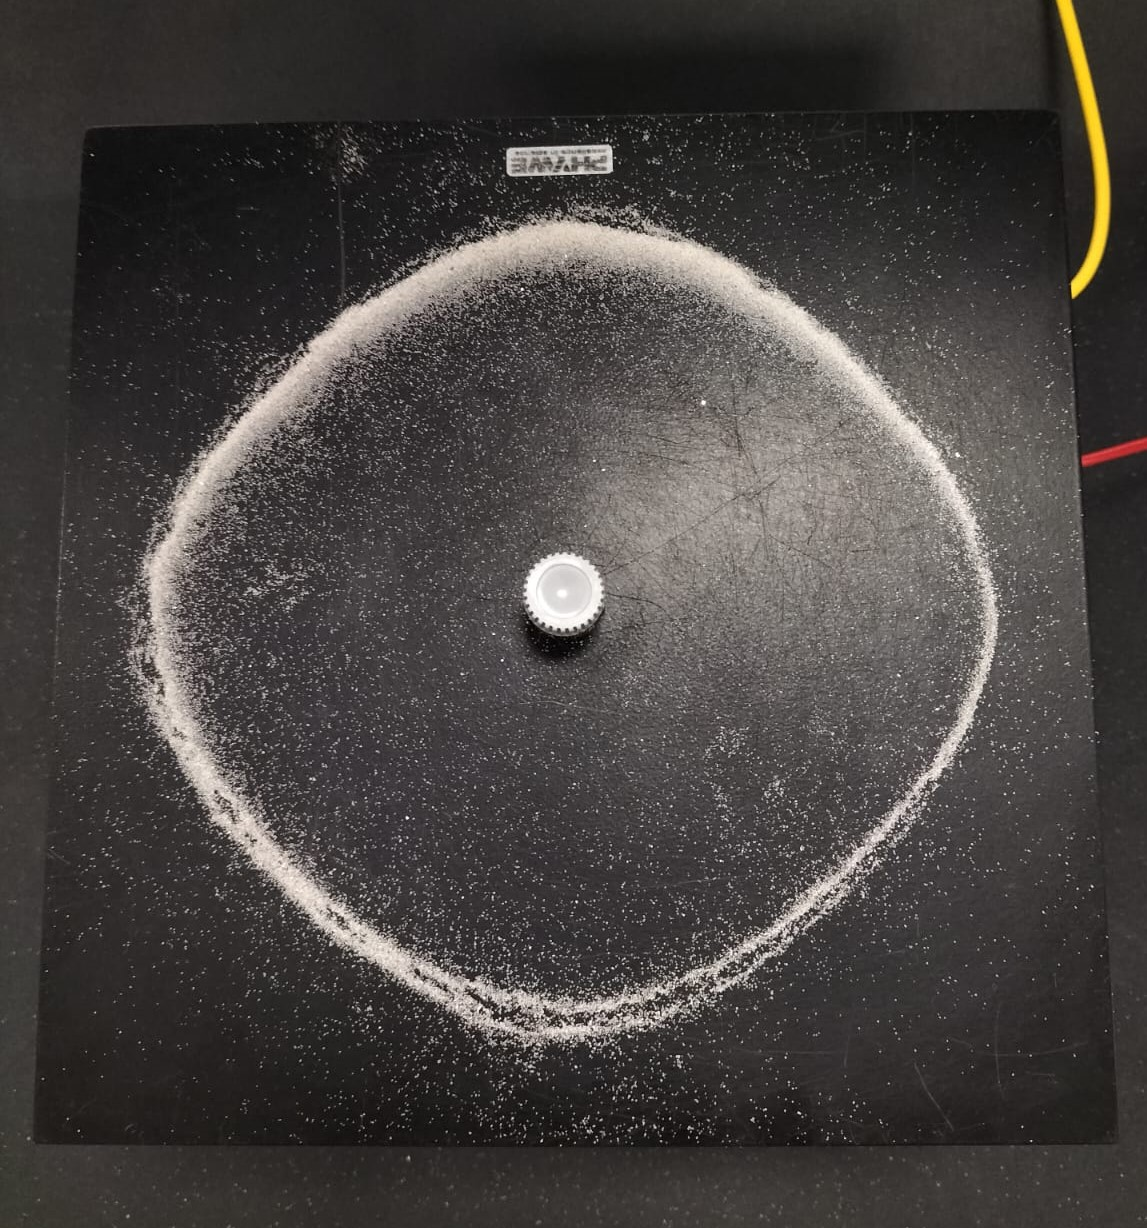
\includegraphics[width=0.4\linewidth]{Images/modo1.jpg}
    \caption{Primer modo normal de la placa cuadrada}
\end{figure}

\newpage

El segundo y último armónico encontrado de la placa cuadrada se produjo a una frecuencia $\nu=539\pm1\;Hz$. Observamos un cuadrado en el centro de la placa y una especie de ramas hiperbólicas en las esquinas, como podemos ver en la imagen:

\begin{figure}[h!]
    \centering
    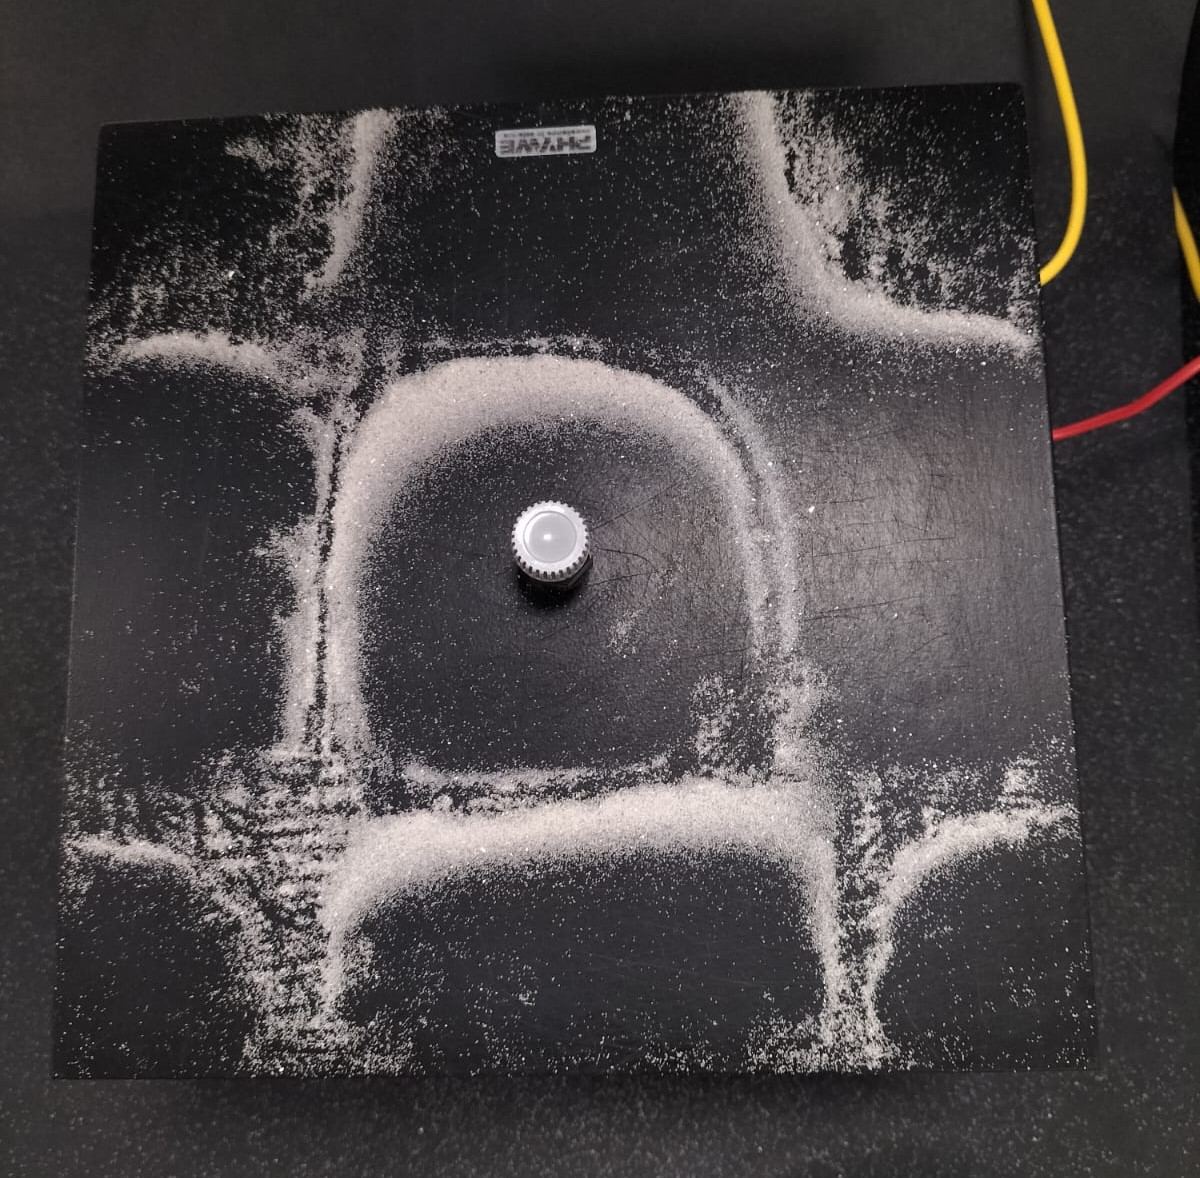
\includegraphics[width=0.4\linewidth]{Images/modo2.jpg}
    \caption{Segundo modo de la placa cuadrada}
\end{figure}

La distribución geométrica de la arena en las diferentes figuras está claramente relacionada con la distribución de nodos y antinodos en la placa. Las zonas en las que se acumula la arena son las líneas nodales, en donde la vibración está cerca de cero, mientras que las zonas en donde no hay arena son aquellas en donde hay más vibración.

\end{document}